\subsection{Trajectory Comparison in Urban Building Layouts}
We further evaluate the frozen planners in urban layouts with variable building heights and stepped profiles. Eight paired seeds generate a base layout of 20 buildings and a denser layout with eight additional infill buildings. Each base building combines a podium with a horizontally offset tower. Podium footprints range from $16\times16$ to $24\times24$ m, with heights of 8--14 m; tower footprints occupy 60\% of each podium side length, with heights of 24--58 m. The infill buildings have side lengths of 10--16 m and heights of 18--42 m. These components form blocks, narrow passages and locally enclosed spaces. Each layout is represented by the union of 40 or 48 axis-aligned boxes. Analytic box checks use a 1 m expansion at each face, and the network clearance features use the minimum component distance. The motion model, candidate library, scheduling parameters and network weights remain fixed. All methods start at $(0,0,20)$ m with an airspeed of $15.5$ m/s and approach $(250,0,20)$ m. The paired comparison comprises 80 nominal closed-loop episodes on 16 maps.

Figure~\ref{fig:urbancomparison} presents the first seed, fixed for both layouts before execution, using the scene-level trajectory comparison format of YOPO~\cite{lu2024yopo}. Buildings are displayed on a 1.5 m voxel grid, while planning and execution checks use the analytic boxes. Every curve connects recorded flight states, including the prefixes of unsuccessful episodes. In the base layouts, Cost, Diverse, Learned, No-geometry and Full complete 7, 6, 4, 8 and 7 of the eight tasks, respectively. With infill development, the corresponding counts decrease to 6, 1, 1, 1 and 4. All methods reach the goal in the displayed base scene; only Cost completes the displayed infill scene, while the other four encounter an inflated building margin. The urban comparison therefore reveals a change in scheduler ranking: the learned ordering advantage observed on the original test families does not extend to these denser building layouts.

\begin{figure*}[!t]
\centering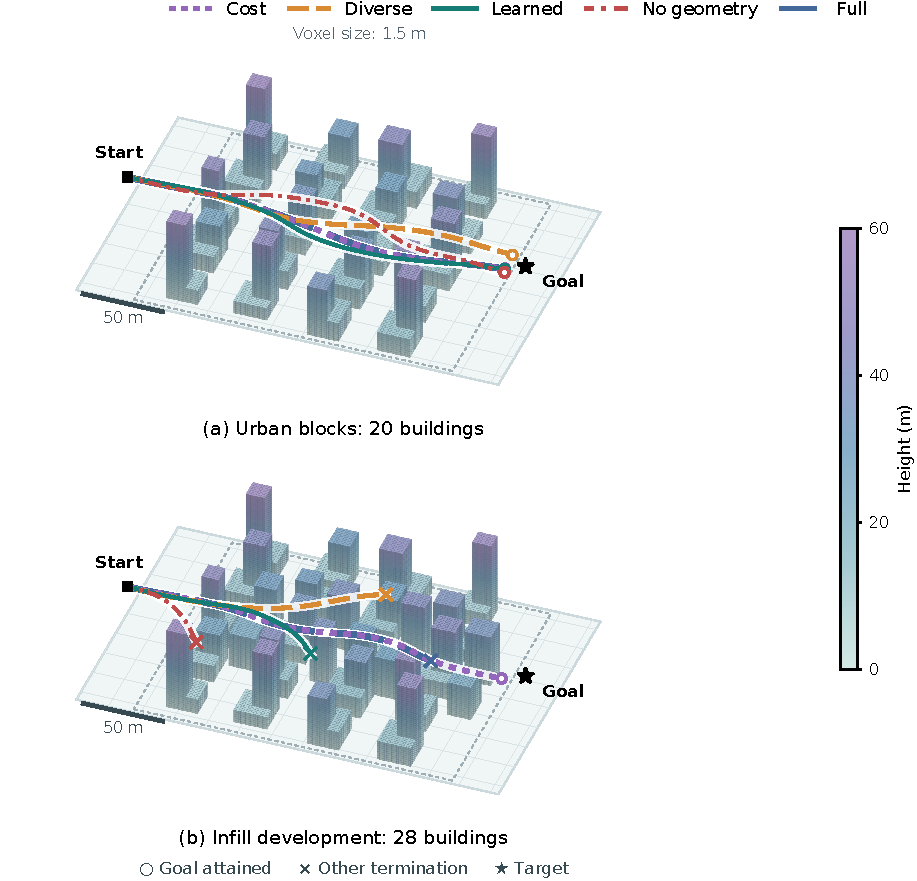
\includegraphics[width=.94\textwidth]{figures/urban_comparison.pdf}
\caption{Nominal closed-loop trajectories in paired urban layouts (seed 701000). The base layout contains 20 podium--tower buildings; infill development retains these buildings and adds eight structures. Height-colored 1.5 m voxels display the physical building volumes. Curves show recorded execution states, circles mark goal attainment, and crosses mark other terminations. All methods use the same analytic box geometry and 1 m face margins.}
\label{fig:urbancomparison}
\end{figure*}
